
\chapter{Appendix - input for interactive UI evaluation}
\label{sec:50_plans}

\begin{figure}
  \centering
  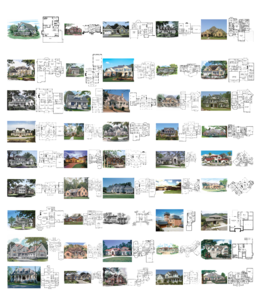
\includegraphics[width=1.0\columnwidth]{fifty_houses_plans.png}
  \caption[The source material for interactive evaluation]{\label{fig:fifty_houses_plans} The input plans and profiles to Fig.~\ref{fig:fifty_1}---\ref{fig:fifty_3}. \copyright 2012 ePlans.}
\end{figure}

\chapter{Appendix - artists' comments on the procedural extrusions system}
\label{sec:artists_comments}

\emph{Please note that the artists refer to the procedural extrusion system as ``the skeleton program'' or similar.}

\subsection{User 1}

{\bf In less than 3 sentences, describe your artistic training (eg: university course and any relevant work experience you've done)}
	My artistic training consists of a bachelors of fine arts degree in 3-D Imaging and Animation from Arizona State University, as well as a certificate in computer gaming. Relevant work experience includes creating all artistic assets for a stroke patient rehabilitation interactive videogame for the Arizona State University Biomedical Research Facility.

{\bf How much programming experience have you had (eg: none? max-scripting? c++?)}
My personal programming experience consists of one meager class in flash programming for videogames that I was not extremely successful at.

{\bf How long did it take you to become competent at using the tool?}
	After being given a list of hot keys and experimenting with the program, it took roughly three weeks to become comfortable with multiple profiles and floor plan pieces while using the program.

{\bf Was the skeleton program easy to use (compare to using Max/Maya/Sketchup)?}
	Compared to Max or Maya the program has a much softer learning curve, from interface aspects to object creation.  For the sole purpose of creating buildings and architecture, the skeleton program appears more expedient than the normal modeling programs due to automated steps it takes in completing and triangulated the meshes.

{\bf How long did it take you to create you current projects (the mansion or the oriental house). How much of this time was creating the meshes. How much of this time was using the skeleton program?}
	To create my brick mansion and final renders took roughly twenty to twenty five hours.  Creating my meshes (windows, door, cornice, chimney) only took about four to five hours in Maya.  It took about 10 hours using the skeleton program to create the mansion mesh itself, but that was due to changing it repeatedly and experimenting with 10+ profiles and how they align.  The latter 10 hours or so was spent in Maya first creating textures, then a 10 piece lighting unit, and then creating quality renders for the paper.

{\bf Would it have taken longer to create these models without the skeleton program? }
Yes, it would have taken quite a while longer to create the mesh in Maya, and I can assume that the triangulation and face count wouldn't be as low either.  It probably would take at least twice the amount of time due to the roof most of all, to create all the angles seamlessly and uniformly.

{\bf Would the tool be a useful addition to current 3D modeling packages?}
	The tool would be very useful for a 3-D Environment modeling package.  Being able to export an OBJ file, it would be very easy to populate the background of an environment with buildings that differed just enough that they didn't look like duplicates, but not so high poly that it would slow down a game engine.

{\bf Any other comments about the skeleton program?}
	Overall the program has quite a lot of potential, if only for a specific set of uses.  The only suggestions I had is to find a way to make the measurements more exact than just the align to grid system, whether it's just a soft grid in the background, or an actual numerical system that can be manipulated.  This goes for the profile view as well.  One thing that makes it very easy in Maya is you can always move things in exact, straight lines, which is very useful for low poly creation.  Occasionally I would find that my building swelled at the top compared the bottom, or one side was actually just a shade shorter than the other even though they look identical on the floor plan.

\subsection{User 2}

{\bf In less than 3 sentences, describe your artistic training (eg: university course and any relevant work experience you've done):}
I have taken a number of traditional art classes including Drawing, Painting, Sculpture, Color Theory as well as 2D and 3D Design. I have also completed 4 classes in 3D Modeling and Animation, and have been using 3D programs for over 5 years. 

{\bf How much programming experience have you had (eg: none? max-scripting? c++?)}
I have taken introductory courses in Visual Basic, C++, Java and Action Script. I am also familiar with HTML and CSS.

{\bf How long did it take you to become competent at using the tool?}
With only the Note document it took me about 5 hours to get a decent understanding of the program. I think that a video guide would cut down on this time quite a bit, as well as give a user a much better grasp of the program.

{\bf Was the skeleton program easy to use (compare to using Max/Maya/Sketchup)?}
Yes, the skeleton program was easy to use compared to Max and Maya.

{\bf How long did it take you to create you current projects (the mansion or oriental house). How much of this time was creating the meshes. How much of this time was using the skeleton program?}
I would say that it took be about 20 to 30 hours to get the oriental house to where it is now.
I would say the majority of this time was spent creating the meshes, 15 to 20 hours and 5 to 10 hours using the skeleton program.


{\bf Would it have taken longer to create these models without the skeleton program?}
I think that it would have taken me longer to get my model to the same level of completion without the skeleton program. I would say traditional modeling techniques would add at least 5 hours of work.

{\bf Would the tool be a useful addition to current 3D modeling packages?}
This would be a great addition to Max or Maya, the speed with which it allows you to create buildings 

{\bf Any other comments about the skeleton program?}
Overall I think that the core idea behind the skeleton program is really great, and for the most part the execution of the program is equally great. The ease with which you can create a building and then tweak it until it is exactly what you are looking for is extremely useful.
In its current state, I think the meshes are the weakest part of the Skeleton program. The main reason I say this is because as it currently stands, the application of meshes doesn’t really save you that much time compared to creating and attaching them within a separate 3D program.
If I were using this program in the industry my preferred pipeline would be something along the lines of the below.

\begin{itemize}
\item{Use the Skeleton program to create the basic shape of a building}
\item{Create any dormer-window like protrusions (if implemented again)}
\item{Apply roof tiles where appropriate within the skeleton program}
\item{Export the building as an .obj file}
\item{Import building into Max or Maya}
\item{Build the detail meshes for the building on top of the imported building}
\item{Duplicate, rotate, and transform the meshes to flesh out all the desired details.}
\end{itemize}

This only difference between the above pipeline and the current pipeline is that currently I build a mesh, skin it, export it, and then attach it within the skeleton program. I think that the removal of the need to skin and weight the meshes makes up for the need to manually duplicate, rotate, and transform them.

Ultimately, in a perfect software, I would love to be able to create meshes and then apply them to my models in a 3D environment instead of the two 2D environment the Skeleton program uses. In other words, I would want the ability to create the anchor points directly on the mesh in the 3D view of the Skeleton program. 

